\chapter{Appendix}
\blindtext

\section{From threshold to per-class probabilities}
\label{sec:appendix:corn_probas}
\blindtext


\section{Adding support for weighting}
\label{sec:appendix:corn_weighting}
% TODO: Reference this section in the main text
\begin{minted}{python}
  loss = -torch.sum(
    (F.logsigmoid(pred)*train_labels
      + (F.logsigmoid(pred) - pred)*(1-train_labels))
    * train_weights # ← new
  )
\end{minted}


\section{Dataset}
\begin{figure}
  \centering
  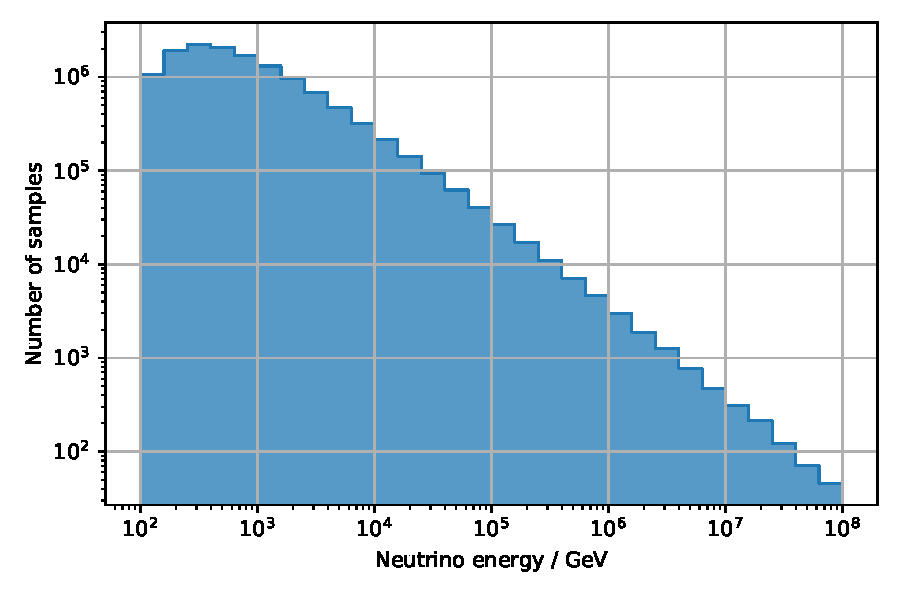
\includegraphics[scale=1]{content/plots/dataset:raw:histogram.pdf}
  \caption{Energy spectrum of the full, untouched Monte-Carlo dataset using 30 bins.}
  \label{fig:dataset:raw:histogram}
\end{figure}

% TODO: Add a table of all features?

\section{Bootstrap distributions}
\begin{figure}
  \centering
  % TODO: correct dimensions
  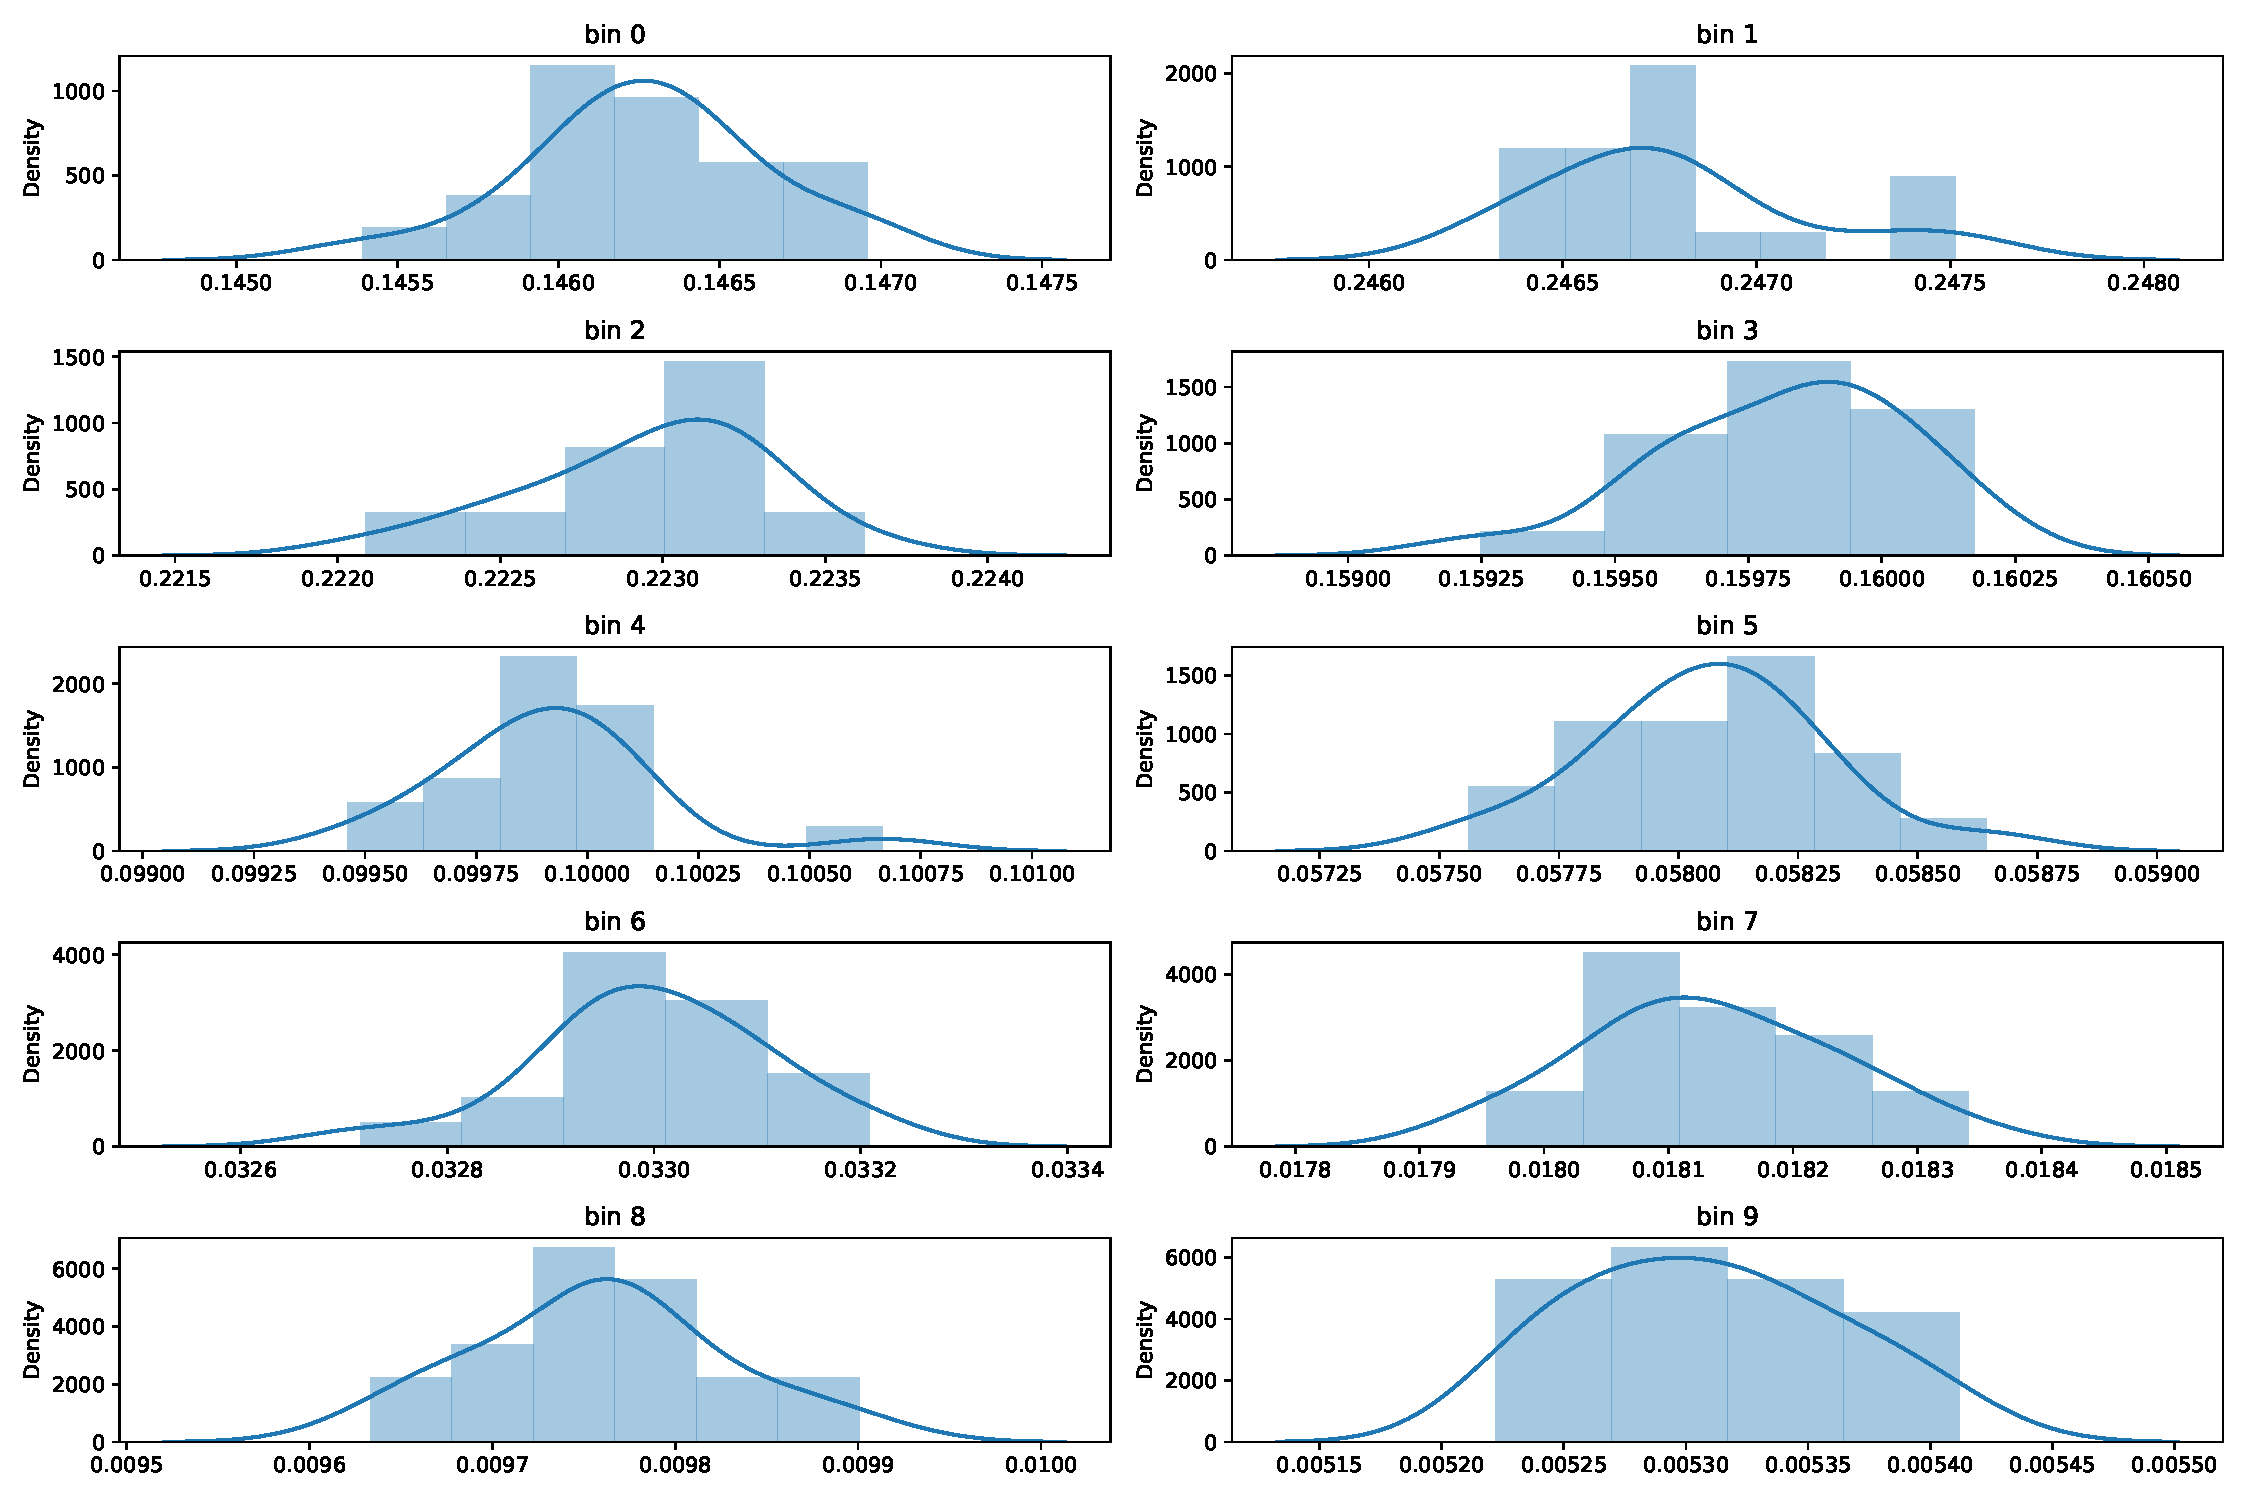
\includegraphics[width=\textwidth]{content/plots/halftime/bootstrap_distributions.pdf}
  \caption{Bootstrap distributions TODO.}
  \label{fig:bootstrap:distributions}
\end{figure}


\section{Links etc.}
\begin{description}
  \item[Dataset in the chair's \texttt{POOL} file system] \texttt{/net/big-tank/POOL/users/lkardum/new\_mc\_binning.csv} (\SI{14.6}{\giga\byte})
  % https://git.e5.physik.tu-dortmund.de/shaefs/bachelor_thesis/
  % https://git.e5.physik.tu-dortmund.de/nweitkemper/ba % TODO: move master → main
\end{description}
% TODO: Link to GitHub / GitLab / code on Phobos
